
\documentclass[border=8pt, multi, tikz]{standalone} 
\usepackage{import}
\subimport{../layers/}{init}
\usetikzlibrary{positioning}
\usetikzlibrary{3d} %for including external image 

\def\ConvColor{rgb:yellow,5;red,2.5;white,5}
\def\ConvReluColor{rgb:yellow,5;red,5;white,5}
\def\PoolColor{rgb:red,1;black,0.3}
\def\UnpoolColor{rgb:blue,2;green,1;black,0.3}
\def\FcColor{rgb:blue,5;red,2.5;white,5}
\def\FcReluColor{rgb:blue,5;red,5;white,4}
\def\SoftmaxColor{rgb:magenta,5;black,7}   
\def\SumColor{rgb:blue,5;green,15}

\newcommand{\copymidarrow}{\tikz \draw[-Stealth,line width=0.8mm,draw={rgb:blue,4;red,1;green,1;black,3}] (-0.3,0) -- ++(0.3,0);}

\begin{document}
\begin{tikzpicture}
\tikzstyle{connection}=[ultra thick,every node/.style={sloped,allow upside down},draw=\edgecolor,opacity=0.7]
\tikzstyle{copyconnection}=[ultra thick,every node/.style={sloped,allow upside down},draw={rgb:blue,4;red,1;green,1;black,3},opacity=0.7]

\node[canvas is zy plane at x=0] (temp) at (-3,0,0) {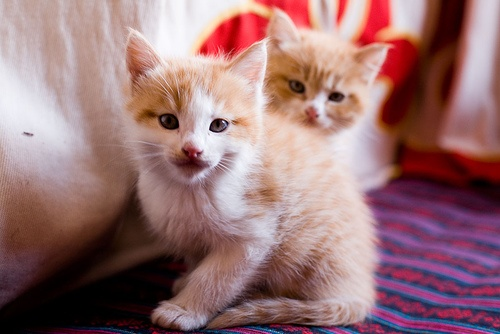
\includegraphics[width=8cm,height=8cm]{../examples/fcn8s/cats.jpg}};

\pic[shift={ (0,0,0) }] at (0,0,0) 
    {RightBandedBox={
        name=SimpleStem,
        caption= ,
        xlabel={{ 64, 64 }},
        zlabel=128,
        fill=\ConvColor,
        bandfill=\ConvReluColor,
        height=40,
        width={ 2 , 2 },
        depth=40
        }
    };

\pic[shift={ (0,0,0) }] at (SimpleStem-east) 
    {Box={
        name=pool_b1,
        caption= ,
        fill=\PoolColor,
        opacity=0.5,
        height=32,
        width=1,
        depth=32
        }
    };

\pic[shift={ (1,0,0) }] at (pool_b1-east) 
    {RightBandedBox={
        name=ccr_VSSBlock_128,
        caption= ,
        xlabel={{ 128, 128 }},
        zlabel=256,
        fill=\ConvColor,
        bandfill=\ConvReluColor,
        height=32,
        width={ 3.5 , 3.5 },
        depth=32
        }
    };

\pic[shift={ (0,0,0) }] at (ccr_VSSBlock_128-east) 
    {Box={
        name=pool_b2,
        caption= ,
        fill=\PoolColor,
        opacity=0.5,
        height=24,
        width=1,
        depth=24
        }
    };

\draw [connection]  (pool_b1-east)    -- node {\midarrow} (ccr_VSSBlock_128-west);

\pic[shift={ (2,0,0) }] at (pool_b2-east) 
    {RightBandedBox={
        name=VisionClueMerge_256,
        caption=VisionClueMerge,
        xlabel={{ 512, 512 }},
        zlabel=32,
        fill=\ConvColor,
        bandfill=\ConvReluColor,
        height=8,
        width={ 8 , 8 },
        depth=8
        }
    };

\draw [connection]  (pool_b2-east)    -- node {\midarrow} (VisionClueMerge_256-west);

\pic[shift={ (1,0,0) }] at (VisionClueMerge_256-east) 
    {RightBandedBox={
        name=ccr_VSSBlock_256,
        caption= ,
        xlabel={{ 256, 256 }},
        zlabel=128,
        fill=\ConvColor,
        bandfill=\ConvReluColor,
        height=25,
        width={ 4.5 , 4.5 },
        depth=25
        }
    };

\pic[shift={ (0,0,0) }] at (ccr_VSSBlock_256-east) 
    {Box={
        name=pool_b3,
        caption= ,
        fill=\PoolColor,
        opacity=0.5,
        height=19,
        width=1,
        depth=19
        }
    };

\draw [connection]  (VisionClueMerge_256-east)    -- node {\midarrow} (ccr_VSSBlock_256-west);

\pic[shift={ (2,0,0) }] at (pool_b3-east) 
    {RightBandedBox={
        name=VisionClueMerge_512,
        caption=VisionClueMerge,
        xlabel={{ 1024, 1024 }},
        zlabel=64,
        fill=\ConvColor,
        bandfill=\ConvReluColor,
        height=8,
        width={ 8 , 8 },
        depth=8
        }
    };

\draw [connection]  (pool_b3-east)    -- node {\midarrow} (VisionClueMerge_512-west);

\pic[shift={ (1,0,0) }] at (VisionClueMerge_512-east) 
    {RightBandedBox={
        name=ccr_VSSBlock_512,
        caption= ,
        xlabel={{ 512, 512 }},
        zlabel=256,
        fill=\ConvColor,
        bandfill=\ConvReluColor,
        height=16,
        width={ 5.5 , 5.5 },
        depth=16
        }
    };

\pic[shift={ (0,0,0) }] at (ccr_VSSBlock_512-east) 
    {Box={
        name=pool_b4,
        caption= ,
        fill=\PoolColor,
        opacity=0.5,
        height=12,
        width=1,
        depth=12
        }
    };

\draw [connection]  (VisionClueMerge_512-east)    -- node {\midarrow} (ccr_VSSBlock_512-west);

\pic[shift={ (2,0,0) }] at (pool_b4-east) 
    {RightBandedBox={
        name=VisionClueMerge_1024,
        caption=VisionClueMerge,
        xlabel={{ 2048, 2048 }},
        zlabel=64,
        fill=\ConvColor,
        bandfill=\ConvReluColor,
        height=8,
        width={ 8 , 8 },
        depth=8
        }
    };

\draw [connection]  (pool_b4-east)    -- node {\midarrow} (VisionClueMerge_1024-west);

\pic[shift={ (1,0,0) }] at (VisionClueMerge_1024-east) 
    {RightBandedBox={
        name=ccr_VSSBlock_1024,
        caption= ,
        xlabel={{ 1024, 1024 }},
        zlabel=512,
        fill=\ConvColor,
        bandfill=\ConvReluColor,
        height=16,
        width={ 5.5 , 5.5 },
        depth=16
        }
    };

\pic[shift={ (0,0,0) }] at (ccr_VSSBlock_1024-east) 
    {Box={
        name=pool_b5,
        caption= ,
        fill=\PoolColor,
        opacity=0.5,
        height=12,
        width=1,
        depth=12
        }
    };

\draw [connection]  (VisionClueMerge_1024-east)    -- node {\midarrow} (ccr_VSSBlock_1024-west);

\pic[shift={ (2,0,0) }] at (pool_b5-east) 
    {RightBandedBox={
        name=DDF_512,
        caption=DDF,
        xlabel={{ 512, 512 }},
        zlabel=128,
        fill=\ConvColor,
        bandfill=\ConvReluColor,
        height=8,
        width={ 8 , 8 },
        depth=8
        }
    };

\draw [connection]  (pool_b5-east)    -- node {\midarrow} (DDF_512-west);

\pic[shift={ (1,0,0) }] at (DDF_512-east) 
    {RightBandedBox={
        name=Upsample_P4,
        caption=Upsample,
        xlabel={{ 128, 128 }},
        zlabel=256,
        fill=\ConvColor,
        bandfill=\ConvReluColor,
        height=40,
        width={ 2 , 2 },
        depth=40
        }
    };

\pic[shift={ (1,0,0) }] at (Upsample_P4-east) 
    {RightBandedBox={
        name=ccr_Concat_P4,
        caption= ,
        xlabel={{ 512, 512 }},
        zlabel=128,
        fill=\ConvColor,
        bandfill=\ConvReluColor,
        height=16,
        width={ 5.5 , 5.5 },
        depth=16
        }
    };

\pic[shift={ (0,0,0) }] at (ccr_Concat_P4-east) 
    {Box={
        name=pool_concat,
        caption= ,
        fill=\PoolColor,
        opacity=0.5,
        height=12,
        width=1,
        depth=12
        }
    };

\draw [connection]  (Upsample_P4-east)    -- node {\midarrow} (ccr_Concat_P4-west);

\pic[shift={ (2,0,0) }] at (pool_concat-east) 
    {RightBandedBox={
        name=Upsample_P3,
        caption=Upsample,
        xlabel={{ 128, 128 }},
        zlabel=256,
        fill=\ConvColor,
        bandfill=\ConvReluColor,
        height=40,
        width={ 2 , 2 },
        depth=40
        }
    };

\pic[shift={ (1,0,0) }] at (Upsample_P3-east) 
    {RightBandedBox={
        name=ccr_Concat_P3,
        caption= ,
        xlabel={{ 256, 256 }},
        zlabel=128,
        fill=\ConvColor,
        bandfill=\ConvReluColor,
        height=16,
        width={ 5.5 , 5.5 },
        depth=16
        }
    };

\pic[shift={ (0,0,0) }] at (ccr_Concat_P3-east) 
    {Box={
        name=pool_concat3,
        caption= ,
        fill=\PoolColor,
        opacity=0.5,
        height=12,
        width=1,
        depth=12
        }
    };

\draw [connection]  (Upsample_P3-east)    -- node {\midarrow} (ccr_Concat_P3-west);

\pic[shift={ (1,0,0) }] at (pool_concat3-east) 
    {RightBandedBox={
        name=Conv_256,
        caption=Conv,
        xlabel={{ 128, 128 }},
        zlabel=256,
        fill=\ConvColor,
        bandfill=\ConvReluColor,
        height=40,
        width={ 3 , 3 },
        depth=40
        }
    };

\pic[shift={ (2,0,0) }] at (pool_concat3-east) 
    {RightBandedBox={
        name=Final_Conv_256,
        caption=Final Conv,
        xlabel={{ 128, 128 }},
        zlabel=256,
        fill=\ConvColor,
        bandfill=\ConvReluColor,
        height=40,
        width={ 3 , 3 },
        depth=40
        }
    };

\pic[shift={(0.75,0,0)}] at (Final_Conv_256-east) 
    {Box={
        name=Softmax_Detection,
        caption=Softmax Detection,
        zlabel=512,
        fill=\SoftmaxColor,
        height=40,
        width=1,
        depth=40
        }
    };

\end{tikzpicture}
\end{document}
